









\begin{frame}
{(Some) counter-measures}
\framesubtitle{Network Reinforcement}
We saw that the main issues for voltage problems are:
\begin{itemize}
    \item Large values of $X_L$
    \item Not enough reactive power compensation
\end{itemize}
To mitigate voltage problems, one solution is to reinforce the network by adding new lines and capacitor banks, static var compensators or synchronous condensers.
\end{frame}

\begin{frame}
{(Some) counter-measures}
\framesubtitle{Voltage regulation}
The second solution is to use the reactive power reserve already available.
In transmission system, we have synchronous machines. They can provide or consume reactive power.
\begin{center}
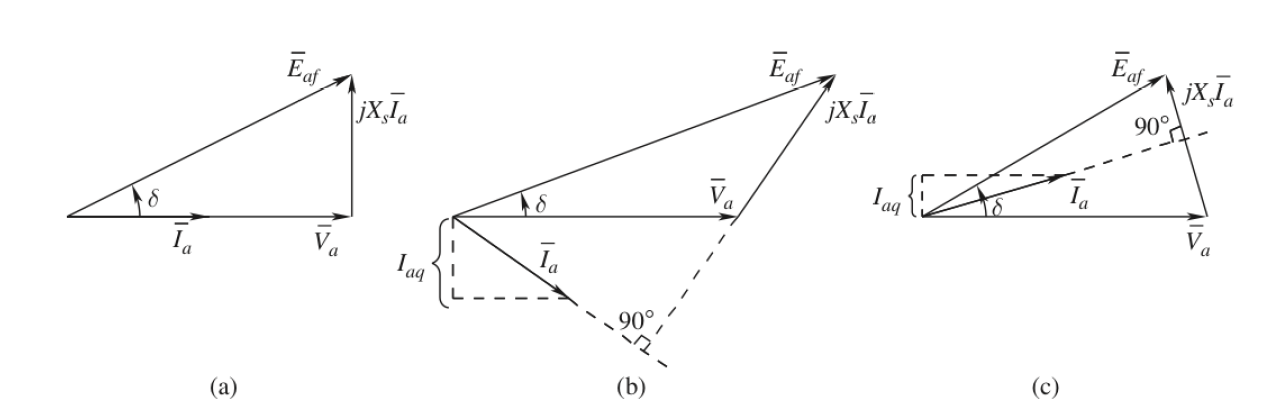
\includegraphics[width=0.9\textwidth]{images/SG_EMF.png}
\end{center}
In this figure $E_{af}$ is the induced emf, $V_a$ the stator voltage, $I_a$ the stator current and $X_s$ the synchronous reactance. In case (a), there is no reactive power transfer. In case (b), the synchronous machine \textbf{provides reactive power} and in case (c), the machine \textbf{consumes reactive power}.
\end{frame}

\begin{frame}
{(Some) counter-measures}
\framesubtitle{Voltage regulation}
\begin{itemize}
    \item When the machine is overexcited, it produces reactive power (because of the larger induced emf).
    \item When it is underexcited, it consumes reactive power.
\end{itemize}
A regulator is responsible for controlling the excitation current in a synchronous generator.
\begin{center}
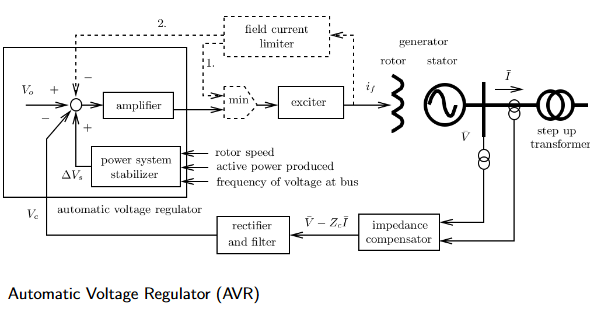
\includegraphics[width=0.8\textwidth]{images/AVR.png}
\end{center}
The voltage setpoints $V_0$ are dispatched by the TSO to ensure a safe and reliable grid.
\end{frame}

\begin{frame}
{Impact of renewable energy resources (RES)}
\framesubtitle{Reverse power flows in distribution systems}
\begin{itemize}
    \item Distribution networks are radial networks (they are built as meshed networks, but operated radially)
    \item Before the venue of distributed energy resources (\emph{PV panels, batteries,...}), the power was flowing from the substation node, down to the end of the feeders.
    \item Increasing penetration of DERs led to reverse power flows.
\end{itemize}
\begin{center}
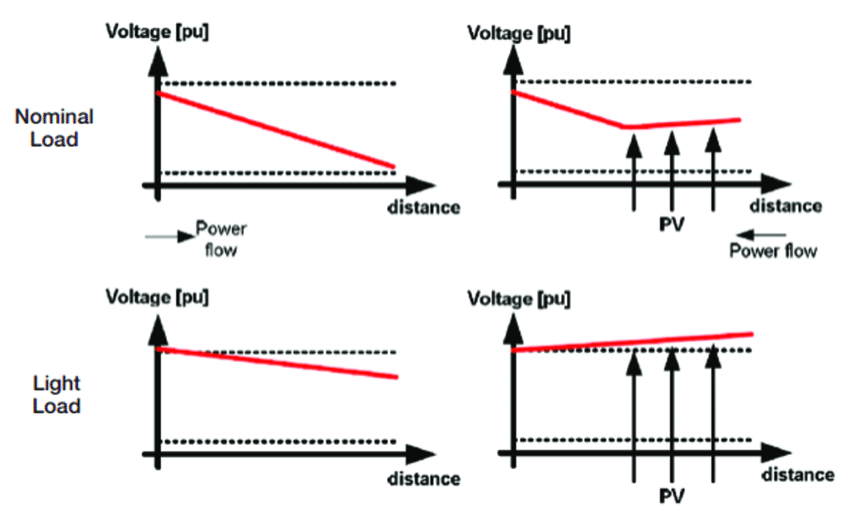
\includegraphics[width=0.7\textwidth]{images/VoltageProfile.png}
\end{center}
\end{frame}

\begin{frame}
{Impact of renewable energy resources (RES)}
\framesubtitle{Reverse power flows in distribution systems}
\begin{itemize}
    \item During hours of high production and low consumption (at midday on a summer day), overvoltages can occur.
    \item It leads to the disconnection of PV inverters $\Rightarrow$ loss of production.
\end{itemize}
\begin{center}
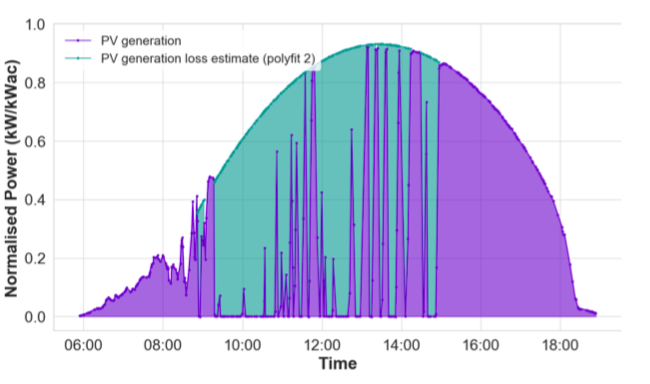
\includegraphics[width=0.6\textwidth]{images/PVdisconnection.png}
\end{center}
\end{frame}

\begin{frame}
{Impact of renewable energy resources (RES)}
\framesubtitle{Reverse power flows in distribution systems}
\begin{itemize}
    \item In distribution systems, the $X/R < 1$. Active power flows have actually a greater influence on voltage magnitudes than reactive power flows.
    \item One way to mitigate overvoltages in distribution networks with high penetration of solar inverters is to do active power curtailment and reactive power compensation.
\end{itemize}
\begin{center}
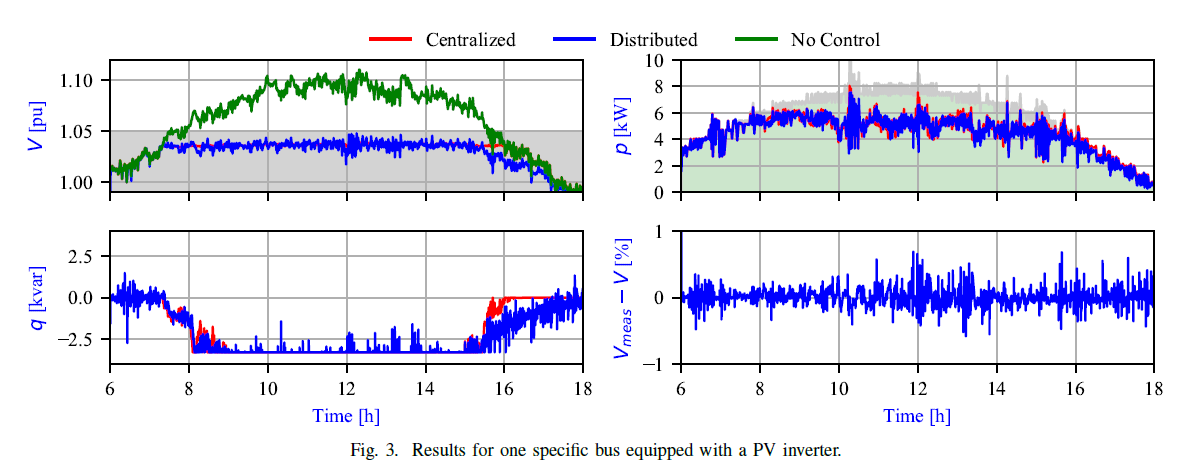
\includegraphics[width=\textwidth]{images/VoltageCtrl.png}
\end{center}
\end{frame}

\begin{frame}
{Impact of renewable energy resources (RES)}
\framesubtitle{Duck Curve}
\begin{itemize}
    \item As we further increase the penetration of RES, changes appear in the demand profile (concept of Duck Curve, now becoming Canyon Curve)
    \item Needs for flexibility to ensure power balance: shut down of flexible production plants when RES start to produce, activate them again when they stop producing
    \item There exist various solutions to \emph{fill the curve}: Demand Side Management, Energy Buffers (e.g. batteries), increasing import/export capacities.
\end{itemize}
\begin{center}
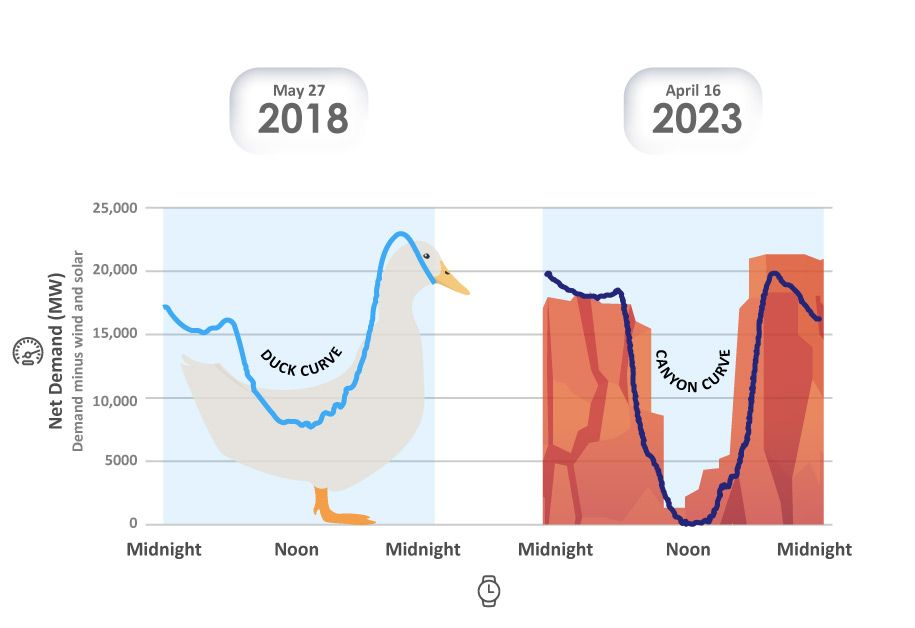
\includegraphics[width=0.6\textwidth]{images/duckcurve.png}
\end{center}
\end{frame}

\begin{frame}
{What did we learn?}
\begin{itemize}
    \item In transmission systems, because lines are inductive $X/R >> 1$, reactive power flows impact voltage magnitudes, and active power flows impact voltage angles.
    \item There is a maximum transmissible power through a line.
    \item Different voltage instabilities, caused by slow acting devices like OLTC (Long-term instabilities), or by faster dynamics like stalling of induction motors (Short-term instabilities).
    \item To prevent voltage instabilities, one can reinforce the grid by adding new lines or new devices, or enforce voltage regulation (local voltage control tracking voltage setpoints given by the system operator).
    \item The increasing penetration of RES creates overvoltage problems in distribution networks and challenges for balancing the system.
\end{itemize